%-----------------------------------------------------------------------------%
\chapter{\topikDua}
%-----------------------------------------------------------------------------%

%-----------------------------------------------------------------------------%
\section{Pendahuluan}
%-----------------------------------------------------------------------------%

OpenCL \textit{Open Computing Language} merupakan \textit{library General Purpose Graphics Processing Unit} Computing (GPGPU) yang dikembangkan oleh Khronos (yang disponsori oleh Apple). OpenCL juga disebut sebagai sebuah \textit{open standard} untuk pemrograman paralel pada sistem heterogen karena mendukung berbagai vendor GPU (\textit{integrated} maupun \textit{dedicated}) seperti Intel, AMD, NVIDIA, Apple dan ARM.

OpenCL merupakan \textit{library} yang dapat berjalan di kebanyakan sistem karena \textit{kernel} bahasanya merupakan subset dari C++ 14. Selain itu, OpenCL juga telah memiliki \textit{language binding} dari bahasa pemrograman \textit{high-level} seperti Microsoft.Net (NOpenCL dan OpenCL.Net), Erlang dan Python (PyOpenCL).

OpenCL saat ini sudah mencapai versi 2.0 dengan sejarah pengembangan \cite{ opencl.mukherjee} sebagai berikut:

\begin{itemize}
	\item OpenCL 1.0​
	\begin{itemize}
		\item Model pemrograman dasar
	\end{itemize}
	\item OpenCL 1.1 and 1.2​
	\begin{itemize}
		\item Teknik manajemen \textit{memory}
		\item Kontrol \textit{resources} yang lebih baik
	\end{itemize}
	\item OpenCL 2.0​
	\begin{itemize}
		\item Memaksimalkan penggunaan kapabilitas baru \textit{hardware}
		\item API pemrograman yang lebih baik
		\item Kontrol \textit{resources} yang lebih baik
	\end{itemize}
\end{itemize}

%-----------------------------------------------------------------------------%
\subsection{Instalasi}
%-----------------------------------------------------------------------------%

Salah satu kelebihan yang dimiliki OpenCL dibanding \textit{hardware-specific library} seperti NVIDIA CUDA adalah dukungan ke banyak vendor \textit{hardware}. Untuk mencapai hal ini, OpenCL beradaptasi dengan karakteristik instalasi masing-masing vendor sehingga setiap vendor memiliki prosedur instalasi OpenCL yang berbeda. Berikut daftar tautan panduan instalasi untuk beberapa vendor ternama:

\begin{itemize}
	\item AMD \url{http://developer.amd.com/tools-and-sdks/opencl-zone​}
	\item Intel \url{https://software.intel.com/en-us/intel-opencl​}
	\item NVIDIA \url{https://developer.nvidia.com/opencl}
\end{itemize}

Contoh langkah-langkah instalasi OpenCL SDK pada Ubuntu 15.10 64-bit dengan NVIDIA 940M \cite{opencl.howto} adalah sebagai berikut:

\begin{enumerate}
	\item Instal \textit{driver} yang disarankan oleh versi Ubuntu 15.10 yaitu NVIDIA \textit{driver} versi 352. Instalasi dapat dilakukan melalui menu \textit{Additional Drivers} atau dengan mengetikkan perintah pada terminal:
	
	\begin{lstlisting}
		
	$ sudo apt-get install nvidia-352
	\end{lstlisting}
	
	\item Setelah itu, instal CUDA dengan mengunduh \textit{repository} CUDA Toolkit versi 7.5 untuk Ubuntu 15.04 (*.deb) di \url{https://developer.nvidia.com/cuda-downloads} dan menjalankan perintah berikut di \textit{terminal}:  
	
	\begin{lstlisting}
	
		$ sudo dpkg -i cuda-repo-ubuntu1504-7-5-*_amd64.deb
		$ sudo apt-get update
		$ sudo apt-get install cuda-toolkit
	\end{lstlisting}
	Pastikan juga baris-baris ini ada di dalam file \verb|~/.bashrc| (baris terbawah):
	
	\begin{lstlisting}
	
		export CUDA_HOME=/usr/local/cuda-7.5 
		export LD_LIBRARY_PATH=${CUDA_HOME}/lib64 
		PATH=${CUDA_HOME}/bin:${PATH} 
		export PATH	
	\end{lstlisting}
	
	Untuk memastikan bahwa driver dan CUDA sudah terinstal sempurna nama GPU (contoh NVIDIA 940M) harus terlihat ketika 2 kelompok perintah ini dipanggil:
	
	Pertama:
	
	\begin{lstlisting}
	
		$ nvidia-smi
	\end{lstlisting}
	
	Kedua:
	
	\begin{lstlisting}
	
		$ cd $CUDA_HOME/samples/1_Utilities/deviceQuery
		$ sudo make run		
	\end{lstlisting}
	
	\item Terakhir, instal header OpenCL dengan perintah:
	
	\begin{lstlisting}
	
	$ sudo apt-get install nvidia-352-dev nvidia-prime nvidia-modprobe nvidia-opencl-dev
	\end{lstlisting}
	
\end{enumerate}

%-----------------------------------------------------------------------------%
\subsection{Struktur Program}
%-----------------------------------------------------------------------------%

Struktur program OpenCL cukup berbeda dengan struktur program CUDA. Perbedaan mendasar adalah adanya proses kompilasi kernel di dalam program OpenCL di mana untuk CUDA proses tersebut tidak perlu dilakukan secara eksplisit pada program. Oleh karena itu, kernel pada program OpenCL biasanya diletakkan di file terpisah dengan ekstensi \verb|*.cl|.

Struktur umum atau langkah-langkah pada program OpenCL adalah sebagai berikut:

\begin{enumerate}
		\item Memilih \textit{platform} yang tersedia
		\item Memilih \textit{device} pada \textit{platform} yang tersedia
		\item Membuat \textit{Context} ​
		\item Membuat \textit{command queue}
		\item Membuat \textit{memory objects} ​
		\item Membaca file \textit{kernel}
		\item Membuat \textit{program object}
		\item Mengkompilasi \textit{kernel}
		\item Membuat \textit{kernel object}
		\item Memasukkan \textit{kernel arguments}
		\item Menjalankan \textit{kernel}
		\item Membaca \textit{memory object} (hasil proses \textit{kernel})
		\item \textit{Free memory objects}
\end{enumerate}

Contoh program sederhana OpenCL \textit{Single-Precision A·X Plus Y} (SAXPY) dapat dilihat pada tautan berikut:

\begin{itemize}
	\item Program utama \url{https://github.com/yohanesgultom/parallel-programming-assignment/blob/master/PR2/opencl/saxpy.c}
	\item Kernel \url{https://github.com/yohanesgultom/parallel-programming-assignment/blob/master/PR2/opencl/saxpy.cl}
\end{itemize}

%-----------------------------------------------------------------------------%
\subsection{Perbandingan Terminologi dengan CUDA}
%-----------------------------------------------------------------------------%

Bagi \textit{programmer} yang sudah terbiasa dengan CUDA, bada bagian ini akan dipaparkan tabel-tabel konversi terminologi antara CUDA dan OpenCL \cite{opencl.cuda.porting}. Dengan tabel-table ini diharapkan \textit{programmer} CUDA dapat lebih cepat memahami OpenCL dan mengkonversi program CUDA ke OpenCL. 

\begin{table}
	\centering
	\caption{Terminologi Perangkat Keras}
	\label{tab:terminologi_perangkat_keras}
	\begin{tabular}{|C{6cm}|C{6cm}|}
		\rowcolor[gray]{.9} \hline \rule[-2ex]{0pt}{5.5ex} CUDA & OpenCL \\ 
		\hline \rule[-2ex]{0pt}{5.5ex} Stream Multiprocessor (SM) & CU (Compute Unit) \\ 
		\hline \rule[-2ex]{0pt}{5.5ex} Thread & Work-item \\ 
		\hline \rule[-2ex]{0pt}{5.5ex} Block & Work-group \\ 
		\hline \rule[-2ex]{0pt}{5.5ex} Global Memory & Global Memory \\ 
		\hline \rule[-2ex]{0pt}{5.5ex} Constant Memory & Constant Memory \\ 
		\hline \rule[-2ex]{0pt}{5.5ex} Shared Memory & Local Memory \\ 
		\hline \rule[-2ex]{0pt}{5.5ex} Local Memory & Private Memory \\ 
		\hline 
	\end{tabular} 
\end{table}

\begin{table}
	\centering
	\caption{Qualifiers untuk fungsi Kernel}
	\label{tab:qualifiers_untuk_fungsi_kernel}
	\begin{tabular}{|C{6cm}|C{6cm}|}
		\rowcolor[gray]{.9} \hline \rule[-2ex]{0pt}{5.5ex} CUDA & OpenCL \\ 
		\hline \rule[-2ex]{0pt}{5.5ex} \verb|_global__ function|​ & \verb|__kernel function| \\ 
		\hline \rule[-2ex]{0pt}{5.5ex} \verb|__device__ function| & N/A \\ 
		\hline \rule[-2ex]{0pt}{5.5ex} \verb|__constant__ variable|​ & \verb|__constant variable| \\ 
		\hline \rule[-2ex]{0pt}{5.5ex} \verb|__device__ variable| & \verb|__global variable| \\ 
		\hline \rule[-2ex]{0pt}{5.5ex} \verb|__shared__ variable| & \verb|__local variable| \\ 
		\hline 
	\end{tabular} 
\end{table}


\begin{table}
	\centering
	\caption{Indeks pada Kernel}
	\label{tab:indeks_pada_kernel}
	\begin{tabular}{|C{6cm}|C{6cm}|}
		\rowcolor[gray]{.9} \hline \rule[-2ex]{0pt}{5.5ex} CUDA & OpenCL \\ 
		\hline \rule[-2ex]{0pt}{5.5ex} \verb|gridDim|​ & \verb|get_num_groups()| \\ 
		\hline \rule[-2ex]{0pt}{5.5ex} \verb|blockDim| & \verb|get_local_size()​| \\ 
		\hline \rule[-2ex]{0pt}{5.5ex} \verb|blockIdx|​ & \verb|get_group_id()| \\ 
		\hline \rule[-2ex]{0pt}{5.5ex} \verb|threadIdx| & \verb|get_local_id()| \\ 
		\hline \rule[-2ex]{0pt}{5.5ex} \verb|blockIdx * blockDim| \newline \verb| + threadIdx| & \verb|get_global_id()| \\ 
		\hline \rule[-2ex]{0pt}{5.5ex} \verb|gridDim * blockDim| & \verb|get_global_size()| \\ 		
		\hline 
	\end{tabular} 
\end{table}

\begin{table}
	\centering
	\caption{Pemanggilan API}
	\label{tab:pemanggilan_api}
	\begin{tabular}{|C{6cm}|C{6cm}|}
		\rowcolor[gray]{.9} \hline \rule[-2ex]{0pt}{5.5ex} CUDA & OpenCL \\ 
		\hline \rule[-2ex]{0pt}{5.5ex} \verb|cudaGetDeviceProperties()|​ & \verb|clGetDeviceInfo()| \\ 
		\hline \rule[-2ex]{0pt}{5.5ex} \verb|cudaMalloc()| & \verb|clCreateBuffer()| \\ 
		\hline \rule[-2ex]{0pt}{5.5ex} \verb|cudaMemcpy()|​ & \verb|clEnqueueReadBuffer()| \newline \verb|clEnqueueWriteBuffer()| \\ 
		\hline \rule[-2ex]{0pt}{5.5ex} \verb|cudaFree()| & \verb|clReleaseMemObj()| \\ 
		\hline \rule[-2ex]{0pt}{5.5ex} \verb|kernel<<<...>>>()| & \verb|clEnqueueNDRangeKernel()| \\ 
		\hline 
	\end{tabular} 
\end{table}

%-----------------------------------------------------------------------------%
\subsection{Library BLAS}
%-----------------------------------------------------------------------------%

\textit{Basic Linear Algebra Subprograms} (BLAS) adalah \textit{library} yang umum digunakan pada pemrograman paralel karena berisi subprogram perkalian matriks dan vektor dasar. BLAS \cite{blas.wiki} awalnya merupakan bagian dari \textit{library} Fortran tetapi kemudian dikembangkan secara terpisah dan terbuka untuk bahasa C dan bahasa lainnya. BLAS terdiri dari 3 tingkat atau kelompok subprogram \cite{blas.netlib}:

\begin{itemize}
	\item Level 1 BLAS: operasi skalar, vektor and vektor-vektor​
	\item Level 2 BLAS: operasi matriks-vektor​
	\item Level 3 BLAS: operasi matriks-matriks
\end{itemize}

OpenCL memiliki beberapa alternatif implementasi BLAS yang dikembangkan oleh beberapa pihak, yaitu:

\begin{enumerate}
	\item ClBLAS
	
	ClBLAS \cite{opencl.clblas} merupakan implementasi \textit{library} BLAS untuk OpenCL yang bersifat \textit{opensource} yang dikembangkan oleh clMath\footnote{https://github.com/clMathLibraries}. \textit{Library} ini sudah mengimplementasikan BLAS secara lengkap (\textit{level} 1, 2 dan 3) dan juga memiliki fitur optimasi khusus untuk AMD GPU. Sisten operasi yang didukung oleh \textit{library} ini adalah Windows ® 7/8​, Linux ​dan Mac OSX. Cara pemanggilan fungsi pada clBLAS dapat dilihat pada gambar \ref{fig:clblas_sgemm}.

	\begin{figure}
		\centering
		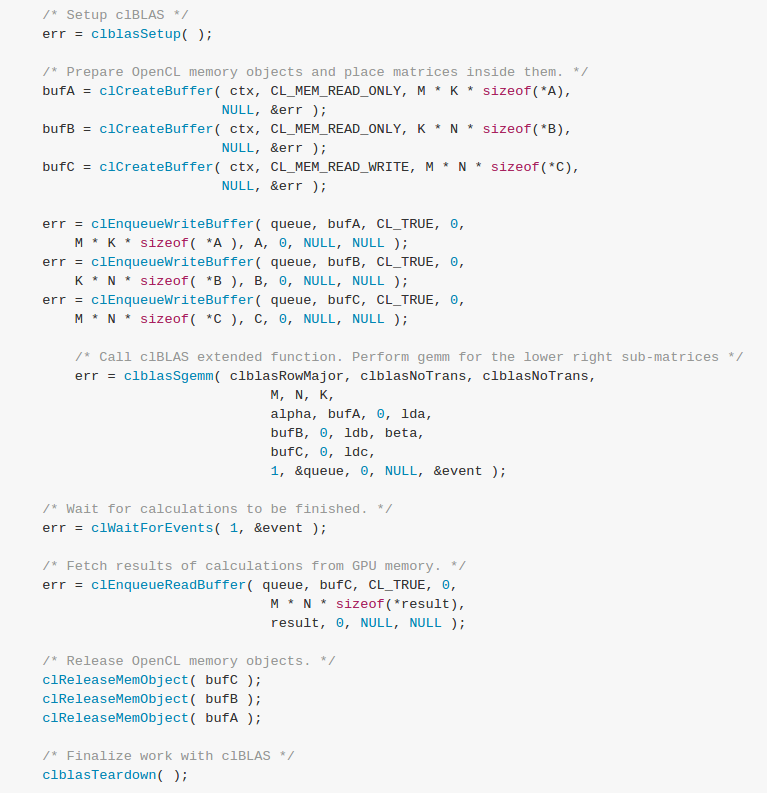
\includegraphics[width=1.0\textwidth]
		{pics/clblas_sgemm.png}
		\caption{Cara pemanggilan clblasSgemm pada clBLAS}
		\label{fig:clblas_sgemm}
	\end{figure}
	
	\item MyGEMM
	
	MyGEMM \cite{opencl.mygemm} adalah \textit{library} yang dikembangkan oleh Cedric Nugteren yang juga bersifat \textit{opensource}. Library ini dikembangkan karena ketidakpuasannya terhadap kinerja clBLAS \cite{opencl.clblas.tutorial} pada NVIDIA GPU. Sekalipun \textit{library} ini dapat dioptimasi untuk NVIDIA GPU, implementasi BLAS yang ada baru \textit{single-precision generalised matrix-multiplication} (SGEMM) saja. Cara pemakaiannya juga sama persis dengan memakai \textit{kernel} OpenCL pada umumnya karena semua fungsi-fungsi BLAS diimplementasikan dalam bentuk file \textit{kernel} OpenCL biasa.	
	
\end{enumerate}

Perbandingan kinerja clBLAS, MyGEMM dan CUBLAS (CUDA) \cite{opencl.clblas.tutorial} pada GPU NVIDIA Tesla K40 dapat dilihat pada gambar \ref{fig:opencl_blas_performance}. Pada grafik tersebut terlihat bahwa kinerja CUDA dengan \textit{library} CUBLAS jauh lebih baik dari semua \textit{library} OpenCL. Di sini Nugteren juga menunjukkan bahwa implentasi SGEMM pada myGEMM lebih baik dari clBLAS.

\begin{figure}
	\centering
	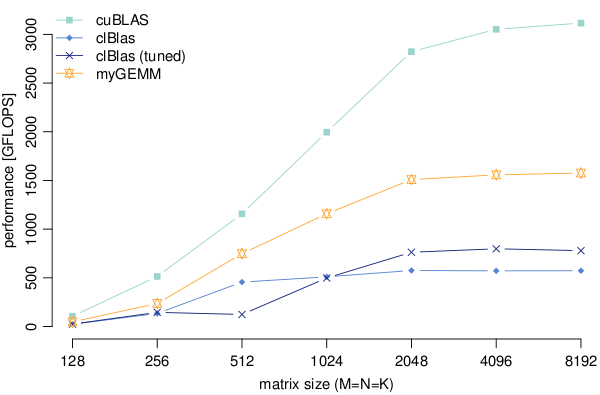
\includegraphics[width=1.0\textwidth]
	{pics/opencl_blas_performance.png}
	\caption{Kinerja library BLAS pada OpenCL}
	\label{fig:opencl_blas_performance}
\end{figure}


%-----------------------------------------------------------------------------%
\subsection{Eksperimen}
%-----------------------------------------------------------------------------%

\subsubsection{Device Query}

OpenCL menyediakan \textit{Application Programming Interface} (API) untuk mengecek \textit{platform} dan \textit{device} OpenCL yang ada di dalam sebuah sistem \cite{opencl.ebook} \cite{opencl.clgetplatforminfo}, yaitu:

\begin{itemize}
	\item \verb|clGetPlatformID()|: mendapatkan daftar \textit{platform} pada mesin
	\item \verb|clGetPlatfrmInfo()|: mendapatkan informasi dari suatu \textit{platform}
	\item \verb|clGetDeviceID()|: mendapatkan daftar \textit{device} pada \textit{platform}
	\item \verb|clGetDeviceInfo()|: mendapatkan informasi dari suatu \textit{device}
\end{itemize}

API ini juga digunakan pada saat menjalankan \textit{kernel} untuk memilih \textit{platform} dan \textit{device} yang ingin digunakan untuk menjalankan \textit{kernel} tersebut.

Pada eksperimen ini, program \verb|device_query.c|\footnote{\url{https://github.com/yohanesgultom/parallel-programming-assignment/blob/master/PR2/opencl/device_query.c}} akan memanggil API untuk mendapatkan informasi \textit{platform} dan \textit{device} kemudian menampilkannya seperti pada gambar \ref{fig:device_query}.

\begin{figure}
	\centering
	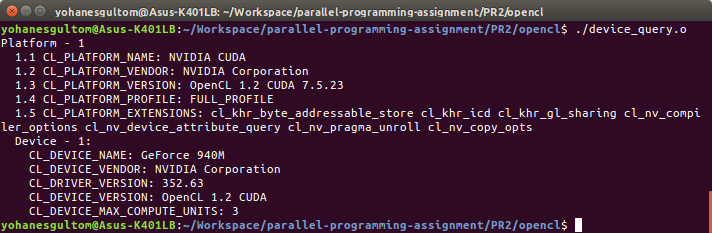
\includegraphics[width=1.0\textwidth]
	{pics/device_query.png}
	\caption{Program untuk mendapatkan informasi platform dan device OpenCL}
	\label{fig:device_query}
\end{figure}

\subsubsection{Single-Precision A·X Plus Y (SAXPY)}

\textit{Single-Precision A·X Plus Y} (SAXPY) adalah program yang melakukan kombinasi perkalian skalar dan penjumlahan vektor $z = \alpha x + y$ di mana $x, y, z$: vektor dan $\alpha$: skalar. Program ini merupakan contoh program yang sederhana tapi cukup merepresentasikan sintaks operasi aljabar linear dari sebuah bahasa program atau \textit{library} sehingga sering dianggap sebagai \textit{"hello world"} untuk program aljabar linear. 

Program SAXPY pada eksperimen ini terdiri dari dua buah file yaitu \verb|saxpy.c|\footnote{\url{https://github.com/yohanesgultom/parallel-programming-assignment/blob/master/PR2/opencl/saxpy.c}} (program utama) dan \verb|saxpy.cl|\footnote{\url{https://github.com/yohanesgultom/parallel-programming-assignment/blob/master/PR2/opencl/saxpy.cl}} (\textit{kernel}). Program ini akan menghitung SAXPY dengan vektor yang berukuran 1.024 elemen dan mencetak hasilnya seperti pada gambar \ref{fig:saxpy}.

\begin{figure}
	\centering
	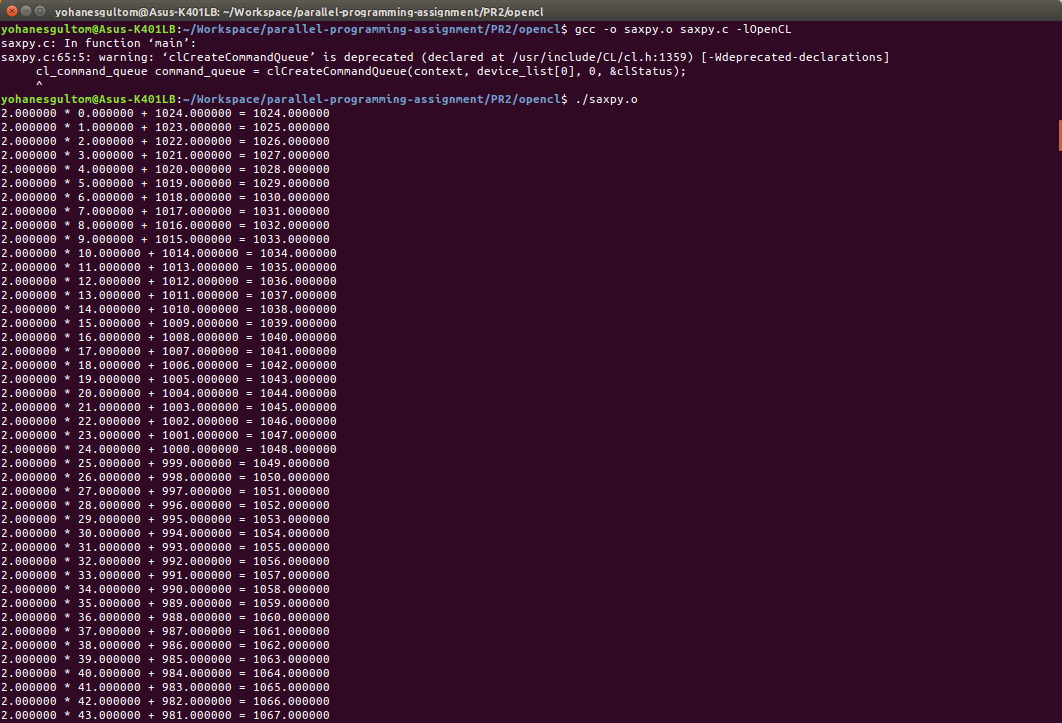
\includegraphics[width=1.0\textwidth]
	{pics/saxpy.png}
	\caption{Program SAXPY 1024 elemen}
	\label{fig:saxpy}
\end{figure}

\subsubsection{Perkalian Matriks Bujursangkar}

Eksperimen ini mencoba membandingkan kinerja perkalian matriks bujursangkar OpenCL \cite{opencl.mmul} dengan CUDA. Program yang digunakan adalah \verb|mmul_cuda.cu|\footnote{\url{https://github.com/yohanesgultom/parallel-programming-assignment/blob/master/PR2/opencl/mmul_cuda.cu}} yang melakukan perkalian matriks bujursangkar dengan CUDA. Sedangkan perkalian matriks bujursangkan OpenCL terdiri dari dua file yaitu \verb|mmul_opencl.c|\footnote{\url{https://github.com/yohanesgultom/parallel-programming-assignment/blob/master/PR2/opencl/mmul_opencl.c}} (program utama) dan \verb|mmul_opencl.cl|\footnote{\url{https://github.com/yohanesgultom/parallel-programming-assignment/blob/master/PR2/opencl/mmul_opencl.c}} (\textit{kernel}).

Hasil eksperimen pada mesin dengan NVIDIA 940M, memberikan hasil seperti grafik pada gambar \ref{fig:mmul_opencl_cuda}. Pada grafik tersebut bahwa untuk ukuran matriks 256x256 sampai 4096x2096, program perkalian matriks dengan OpenCL selalu sedikit lebih lambat dari program yang dibuat dengan CUDA. Sekalipun demikian untuk kasus ini, perbedaan kecepatan antara OpenCL dan CUDA sangatlah kecil, yaitu di bawah 0.3 detik.

\begin{figure}
	\centering
	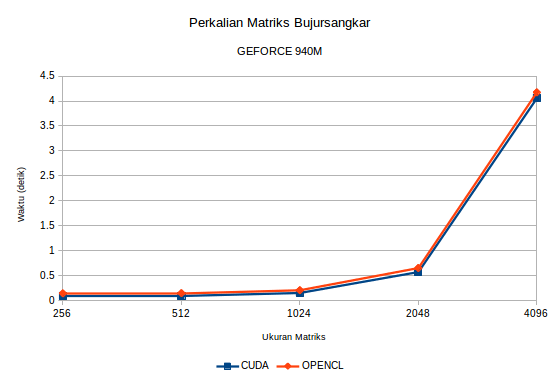
\includegraphics[width=1.0\textwidth]
	{pics/mmul_opencl_cuda.png}
	\caption{Perbandingan perkalian matriks bujursangkar OpenCL dengan CUDA}
	\label{fig:mmul_opencl_cuda}
\end{figure}

\subsubsection{Gaussian Filter Blurring pada Gambar Bitmap}

\textit{Gaussian filter blurring} adalah teknik untuk membuat gambar menjadi \textit{blur} (kabur) (seperti gambar \ref{fig:blur_result}) dengan memanfaatkan perkalian dengan matriks yang dibangun menggunakan persamaan Gaussian \ref{eq:gaussian}.

\noindent \begin{align}\label{eq:gaussian}
g(x,y) = \frac{1}{2\pi \sigma^2} \cdot e^{-\frac{x^2 + y^2}{2 \sigma^2}}
\end{align}

\begin{figure}
	\centering
	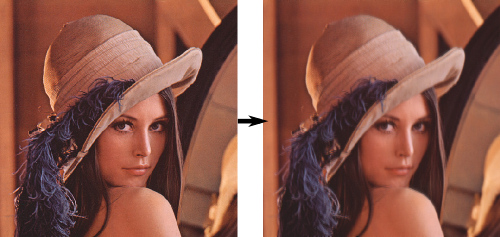
\includegraphics[width=0.5\textwidth]
	{pics/blur_result.png}
	\caption{Proses Gaussian Filter Blurring pada gambar}
	\label{fig:blur_result}
\end{figure}

Eksperimen ini mencoba membandingkan kinerja Gaussian \textit{bluring} dengan CPU dan dengan GPU (menggunakan OpenCL) \cite{opencl.gaussianblur}. Program yang digunakan terdiri dari kumpulan \textit{library file}\footnote{\url{https://github.com/yohanesgultom/parallel-programming-assignment/tree/master/PR2/opencl/OpenCL_Gaussian_Blur}} dengan file utama \verb|main.c| (program utama) dan \verb|kernel.cl| (\textit{kernel}) yang akan melakukan Gaussian \textit{blurring} dengan CPU dan GPU serta menghitung waktu eksekusinya.

\begin{figure}
	\centering
	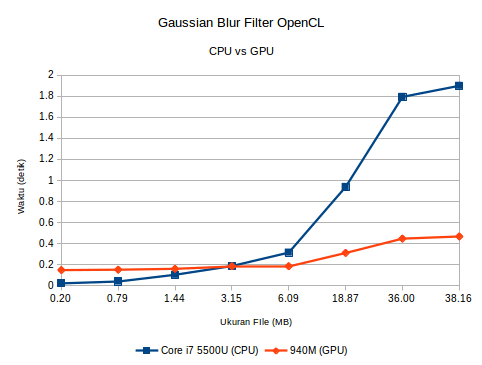
\includegraphics[width=1.0\textwidth]
	{pics/gaussian_blur_cpu_gpu.png}
	\caption{Kinerja Gaussian Blurring CPU vs GPU}
	\label{fig:gaussian_blur_cpu_gpu}
\end{figure}

Hasil eksperimen yang dilakukan menggunakan gambar BMP dengan ukuran 0,2 MB - 38,16 MB memberikan hasil seperti grafik pada gambar \ref{fig:gaussian_blur_cpu_gpu}. Pada hasil eksperimen tersebut terlihat bahwa pada gambar BMP dengan ukuran di bawah 3,15 MB, CPU (Intel Core i7 5500U) dapat melakukan Gaussian \textit{blurring} lebih cepat dari GPU (NVIDIA 940M). Tetapi ketika gambar BMP yang diproses sudah lebih besar dari 3,15 MB, terlihat bahwa GPU dapat menyelesaikan proses dengan lebih cepat. Bahkan untuk ukuran gambar paling besar (38,16 MB), waktu yang dibutuhkan GPU untuk melakukan blurring hanya 0,4 detik atau sekitar $\nicefrac{1}{5}$ dari waktu yang dibutuhkan CPU.